\begin{titlepage}	% начало титульной страницы

	\begin{center}		% выравнивание по центру

		\large Санкт-Петербургский Политехнический Университет Петра Великого\\
		\large Институт компьютерных наук и технологий \\
		\large Кафедра компьютерных систем и программных технологий\\[1cm]
		% название института, затем отступ 6см
		
		\begin{figure}[H]
			\begin{center}
				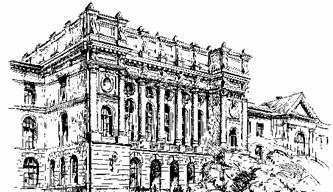
\includegraphics[scale=0.7]{pictures/spbpu.jpg}
			\end{center}
		\end{figure}		
		
		\huge Арифметические и логические основы вычислительной техники\\[0.5cm] % название работы, затем отступ 0,5см
		\large Программная реализация представления числа в различных системах счисления\\[11cm]

	\end{center}


	\begin{flushright} % выравнивание по правому краю
		\begin{minipage}{0.25\textwidth} % врезка в половину ширины текста
			\begin{flushleft} % выровнять её содержимое по левому краю

				\large\textbf{Работу выполнил:}\\
				\large Ламтев А.Ю.\\
				\large {Группа:} 23501/4\\

			\end{flushleft}
		\end{minipage}
	\end{flushright}
	
	\vfill % заполнить всё доступное ниже пространство

	\begin{center}
	\large Санкт-Петербург\\
	\large \the\year % вывести дату
	\end{center} % закончить выравнивание по центру

\thispagestyle{empty} % не нумеровать страницу
\end{titlepage} % конец титульной страницы

\vfill % заполнить всё доступное ниже пространство
